%
\edef\maxSat{MAX-SAT}%
\edef\maxTSat{MAX-3SAT}%
\def\oFlip{\ensuremath{1}-flip}%
\def\tFlip{\ensuremath{2}-flip}%
\def\mFlip{\ensuremath{m}-flip}%
%
\section{Example: \maxSat}%
%
%%
\gdef\maxSatClauses{\textcolor{red}{\ensuremath{k}}}%
\gdef\maxSatVariables{\textcolor{green}{\ensuremath{n}}}%
\gdef\maxSatVariable{\ensuremath{x}}%
\gdef\maxSatVariablei#1{\ensuremath{\maxSatVariable_{#1}}}%
\gdef\maxSatFormula{\ensuremath{B}}%
%%
\begin{frame}[t]%
\frametitle{\maxSat}%
\begin{itemize}%
\item Satisfiability Problems (SAT)\uncover<2->{:%
\begin{itemize}
\item The satisfiability problem (SAT) is one of the most prominent problems in artificial intelligence, logic, theoretical computer science, and various application areas.\scitep{HS2000SAORFROS}%
\item<3-> Given: formula \maxSatFormula\ in Boolean logic consisting of \maxSatVariables\ Boolean variables $\vec{\maxSatVariable}=(\maxSatVariablei{1}, \maxSatVariablei{2}, \dots, \maxSatVariablei{\maxSatVariables})^T$ which each can be either \texttt{true} or \texttt{false}%
\item<4-> Goal: find a setting for these variables so that $\maxSatFormula$ becomes \texttt{true}%
\item<5-> \maxSatFormula\ consists of \maxSatClauses\ clauses which are combined with \inQuotes{$\land$}%
\end{itemize}%
}%
%
\item<6-> \maxSat\uncover<7->{%
\begin{itemize}%
\item SAT turned into an optimization problem\scitep{HS2005SLSFAA}%
\item<8-> candidate solution: bit string of length \maxSatVariables\ holding the value of each variable%
\item<9-> make as many clauses become \texttt{true} as possible%
\item<10-> minimize objective function $\objectiveFunctionb{\vec{x}} = \textnormal{number of clauses which are \texttt{false}}$%
\item<11-> $\objectiveFunctionb{\vec{x}}=0$ $\Longrightarrow$ all clauses are \texttt{true}, SAT problem solved%
\item<12-> $\objectiveFunctionb{\vec{x}}=\maxSatClauses$ $\Longrightarrow$ all clauses are \texttt{false}%
\end{itemize}%
}%
%
\end{itemize}%
%
\locateGraphic{-5}{width=0.55\paperwidth}{graphics/problem_examples/sat/sat}{0.225}{0.54}%
%
\end{frame}%
%
\begin{frame}[t]%
\frametitle{Investigated Algorithms}%
\begin{itemize}%
\item We want to compare the performance of six algorithms\uncover<2->{:%
\begin{enumerate}%
\item 1-flip Hill Climber\only<-2>{: starts with a random bit string, flips one of the \maxSatVariables\ bits in each iteration and keeps the new bit string if it is better}%
\item<3-> 1-flip Hill Climber with Restarts\only<3>{ after $z$ moves without improvements; initially $z=1$ and increased by~$1$ after each restart}%
\item<4-> 2-flip Hill Climber%
\item<5-> 2-flip Hill Climber with Restarts%
\item<6-> $m$-flip Hill Climber\only<6>{, $m$ chosen randomly according to geometric distribution}%
\item<7-> $m$-flip Hill Climber with Restarts%
%
\end{enumerate}%
}%
\item<8-> \alert{Which of these algorithms performs best? When? Why?}%
\end{itemize}%
\end{frame}%
%
\begin{frame}%
\frametitle{Benchmark}%
\begin{itemize}%
\item As benchmark, we use \emph{some} instances from \satLib\expandafter\scitep{\satLibReferences}\uncover<2->{:%
\begin{center}%
\medskip%
\begin{small}%
\begin{tabular}{|l|r|r||l|r|r|}%
\hline%
\textbf{Instance Set} & \textbf{\ensuremath{\mathbf{\maxSatVariables}}} & \textbf{\ensuremath{\mathbf{\maxSatClauses}}}&\textbf{Instance Set} & \textbf{\ensuremath{\mathbf{\maxSatVariables}}} & \textbf{\ensuremath{\mathbf{\maxSatClauses}}}\\%
\hline%
\texttt{uf020}&20&91&\texttt{uf150}&150&645\\%
\texttt{uf050}&50&218&\texttt{uf175}&175&753\\%
\texttt{uf075}&75&325&\texttt{uf200}&200&860\\%
\texttt{uf100}&100&430&\texttt{uf225}&225&960\\%
\texttt{uf125}&125&538&\texttt{uf250}&250&1065\\%
\hline%
\end{tabular}%
\medskip%
\end{small}%
\end{center}%
}%
\item<3-> We pick the first ten instances from each set, i.e., test 100 instances in total%
%\item<4-> All instances are satisfiable%
%\item<5-> The problem instances have the following features\uncover<6->{:%
%\begin{itemize}%
%\item \maxSatVariables: the number of variables%
%\item<7-> \maxSatClauses: the number of clauses (here related to \maxSatVariables)%
%\end{itemize}%
%}%
\end{itemize}%
\end{frame}%
%
%
\begin{frame}[t]%
\frametitle{Example of Log File}%
%
\begin{itemize}%
\only<-1>{\item Now we do experiments and collect data.}%
\item<2-> Example log file obtained from applying the 2-flip Hill Climber with Restarts to the 2\textsuperscript{nd} benchmark instance of set \texttt{uf075}.%
\end{itemize}%
%
\begin{locateBox}[2-]{0.25}{0.235}
\begin{listingBlock}[0.65]{Log File \texttt{uf075-02\_2FlipHCrs\_01.txt}.}
\centering
\begin{scaledBox}{!}{0.3\paperheight}
\lstinputlisting[tabsize=17]{graphics/maxsat_example/exampleMaxSatLogFile.txt}
\end{scaledBox}
\end{listingBlock}
\end{locateBox}
%
\begin{locateBox}[3-]{0}{0}
\begin{pgfpicture}%
\pgfpathrectangle{\pgfpoint{0pt}{0pt}}{\pgfpoint{\paperwidth}{\paperheight}}%
\pgfusepath{use as bounding box,clip}%
%
\pgfsetcolor{blue}%
\pgftext[right,bottom,at=\pgfpoint{0.2\paperwidth}{0.55\paperheight}]{log point}%
\pgfsetlinewidth{1pt}%
\pgfpathmoveto{\pgfpoint{0.21\paperwidth}{0.56\paperheight}}%
\pgfpathlineto{\pgfpoint{0.32\paperwidth}{0.525\paperheight}}%
\pgfusepath{stroke}%
\pgfsetlinewidth{2pt}%
\pgfpathrectangle{\pgfpoint{0.32\paperwidth}{0.51\paperheight}}{\pgfpoint{0.52\paperwidth}{0.03\paperheight}}%
\pgfusepath{stroke}%
%
\uncover<4->{%
%
\pgfsetcolor{red}%
\pgftext[right,bottom,at=\pgfpoint{0.2\paperwidth}{0.45\paperheight}]{ellapsed \measureFEs}%
\pgfsetlinewidth{1pt}%
\pgfpathmoveto{\pgfpoint{0.21\paperwidth}{0.46\paperheight}}%
\pgfpathlineto{\pgfpoint{0.36\paperwidth}{0.4\paperheight}}%
\pgfusepath{stroke}%
\pgfsetlinewidth{2pt}%
\pgfpathrectangle{\pgfpoint{0.36\paperwidth}{0.085\paperheight}}{\pgfpoint{0.1\paperwidth}{0.585\paperheight}}%
\pgfusepath{stroke}%
%
\uncover<5->{%
\pgfsetcolor{green}%
\pgftext[right,bottom,at=\pgfpoint{0.2\paperwidth}{0.35\paperheight}]{runtime [\nano\second]}%
\pgfsetlinewidth{1pt}%
\pgfpathmoveto{\pgfpoint{0.21\paperwidth}{0.365\paperheight}}%
\pgfpathlineto{\pgfpoint{0.56\paperwidth}{0.3\paperheight}}%
\pgfusepath{stroke}%
\pgfsetlinewidth{2pt}%
\pgfpathrectangle{\pgfpoint{0.56\paperwidth}{0.085\paperheight}}{\pgfpoint{0.11\paperwidth}{0.585\paperheight}}%
\pgfusepath{stroke}%
%
\uncover<6->{%
\pgfsetcolor{violet}%
\pgftext[right,bottom,at=\pgfpoint{0.2\paperwidth}{0.25\paperheight}]{\measureObjectiveValue: best \objectiveFunctionb{\vec{x}}}%
\pgfsetlinewidth{1pt}%
\pgfpathmoveto{\pgfpoint{0.21\paperwidth}{0.26\paperheight}}%
\pgfpathlineto{\pgfpoint{0.7\paperwidth}{0.2\paperheight}}%
\pgfusepath{stroke}%
\pgfsetlinewidth{2pt}%
\pgfpathrectangle{\pgfpoint{0.7\paperwidth}{0.085\paperheight}}{\pgfpoint{0.1\paperwidth}{0.585\paperheight}}%
\pgfusepath{stroke}%
}}}%
\end{pgfpicture}%
\end{locateBox}%
%
\end{frame}
%
\begin{frame}[t]{Obtained Data}%
\def\shortcutForAfterExperimentText{e have $6*20*10*10=\numprint{12000}$ log files\only<-6>{!}\uncover<7->{ (with $\numprint{607993}$ log points and $8.6~\mebi\byte$ total)!}}%
\parbox[t]{0.6\paperwidth}{%
\bigskip%
\begin{itemize}%
\item OK, so after the experiment\only<-7>{\dots%
\uncover<2->{%
\begin{itemize}%
\item {\dots}we have $20$ independent runs (log files)%
\item<3-> for each of the $6$ algorithm setups,%
\item<4-> on each of the $10$ benchmark instances%
\item<5-> of each of the $10$ instance sets.%
\item<6-> W\shortcutForAfterExperimentText%
\end{itemize}%
}%
}%
\only<8->{ w\shortcutForAfterExperimentText}%
\item<9-> \alert<-9>{How can we extract useful information from them\only<-8>{?}%
\uncover<10->{ in order to answer the questions which algorithm performs best, when, and why?}}%
\item<11-> What you most likely do: Write your own small program.%
\item<12-> What you now can do: Use our \optimizationBenchmarking\ evaluator!%
\end{itemize}%
}%
%
\locate{2-}{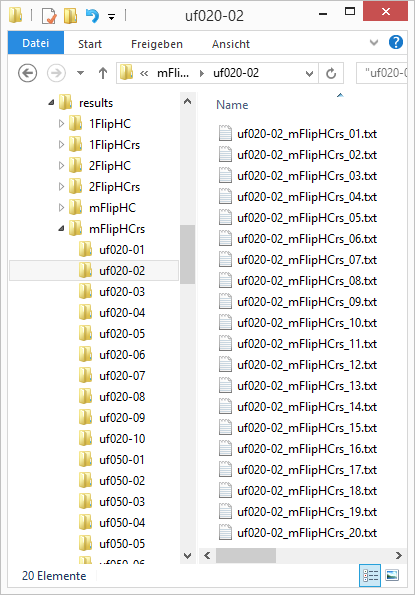
\includegraphics[width=0.33\paperwidth]{graphics/maxsat_example/maxsat_example_log_file_folder_structure}}{0.65}{0.21}%
%
\begin{locateBox}[2-5]{0.65}{0.21}
\begin{pgfpicture}%
\pgfpathrectangle{\pgfpoint{0pt}{0pt}}{\pgfpoint{0.33\paperwidth}{0.79\paperheight}}%
\pgfusepath{use as bounding box,clip}%
%
\pgfsetcolor{alertviolet}%
\pgfsetlinewidth{0.5pt}%
%
\only<3>{%
\pgfpathrectangle{\pgfpoint{0.05\paperwidth}{0.649\paperheight}}{\pgfpoint{0.07\paperwidth}{0.02\paperheight}}%
\pgfpathrectangle{\pgfpoint{0.05\paperwidth}{0.626\paperheight}}{\pgfpoint{0.07\paperwidth}{0.02\paperheight}}%
\pgfpathrectangle{\pgfpoint{0.05\paperwidth}{0.603\paperheight}}{\pgfpoint{0.07\paperwidth}{0.02\paperheight}}%
\pgfpathrectangle{\pgfpoint{0.05\paperwidth}{0.580\paperheight}}{\pgfpoint{0.07\paperwidth}{0.02\paperheight}}%
\pgfpathrectangle{\pgfpoint{0.05\paperwidth}{0.557\paperheight}}{\pgfpoint{0.07\paperwidth}{0.02\paperheight}}%
\pgfpathrectangle{\pgfpoint{0.05\paperwidth}{0.534\paperheight}}{\pgfpoint{0.07\paperwidth}{0.02\paperheight}}%
}%
%
\only<2>{%
\pgfpathrectangle{\pgfpoint{0.272\paperwidth}{0.21\paperheight}}{\pgfpoint{0.018\paperwidth}{0.445\paperheight}}%
\pgfpathrectangle{\pgfpoint{0.013\paperwidth}{0.17\paperheight}}{\pgfpoint{0.06\paperwidth}{0.02\paperheight}}%
}%
%
\only<4>{%
\pgfpathrectangle{\pgfpoint{0.06\paperwidth}{0.319\paperheight}}{\pgfpoint{0.06\paperwidth}{0.212\paperheight}}%
}%
%
\only<5>{%
\pgfpathrectangle{\pgfpoint{0.06\paperwidth}{0.513\paperheight}}{\pgfpoint{0.0433\paperwidth}{0.02\paperheight}}%
\pgfpathrectangle{\pgfpoint{0.06\paperwidth}{0.2958\paperheight}}{\pgfpoint{0.0433\paperwidth}{0.02\paperheight}}%
}%
%
\pgfusepath{stroke}%
%
\end{pgfpicture}%
\end{locateBox}%
\end{frame}%
%
\begin{frame}[label=maxSatInteractiveDemoStart]%
\frametitle{Demo}%
\centering\alert{\textbf{\LARGE{Demo}}}%
\bigskip%
\begin{itemize}%
\item the evaluator GUI%
\item the structure of the data%
\item running an evaluation process%
\item viewing the results% 
\end{itemize}%
\bigskip%
\centering\scalebox{1.8}{\hyperlink{maxSatDemoStart}{\beamergotobutton{go to static demo slides}}}%
\locateGraphic{}{width=0.2\paperwidth}{graphics/logo/logo}{0.725}{0.65}%
\end{frame}%
%
%
\begin{frame}[b,label=maxSatInteractiveDemoEnd]%
\frametitle{The Flow}%
%
\only<-1>{%
\strut\vfill\strut%
\centering{\LARGE{\textbf{\alert{The evaluator works as follows\dots}}}}%
\strut\vfill\strut%
}%
%
\locate{2-3}{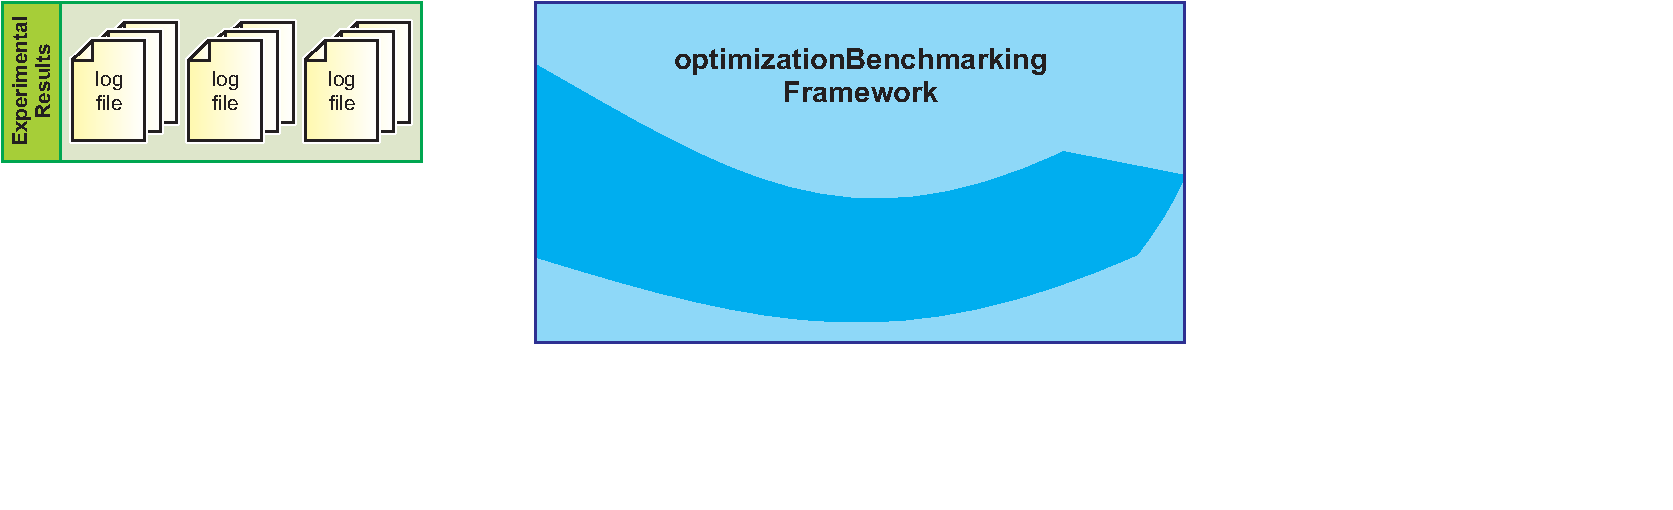
\includegraphics[width=0.9\paperwidth]{graphics/flow/flow_input_1_results}}{0.05}{0.16}%
\locate{4-5}{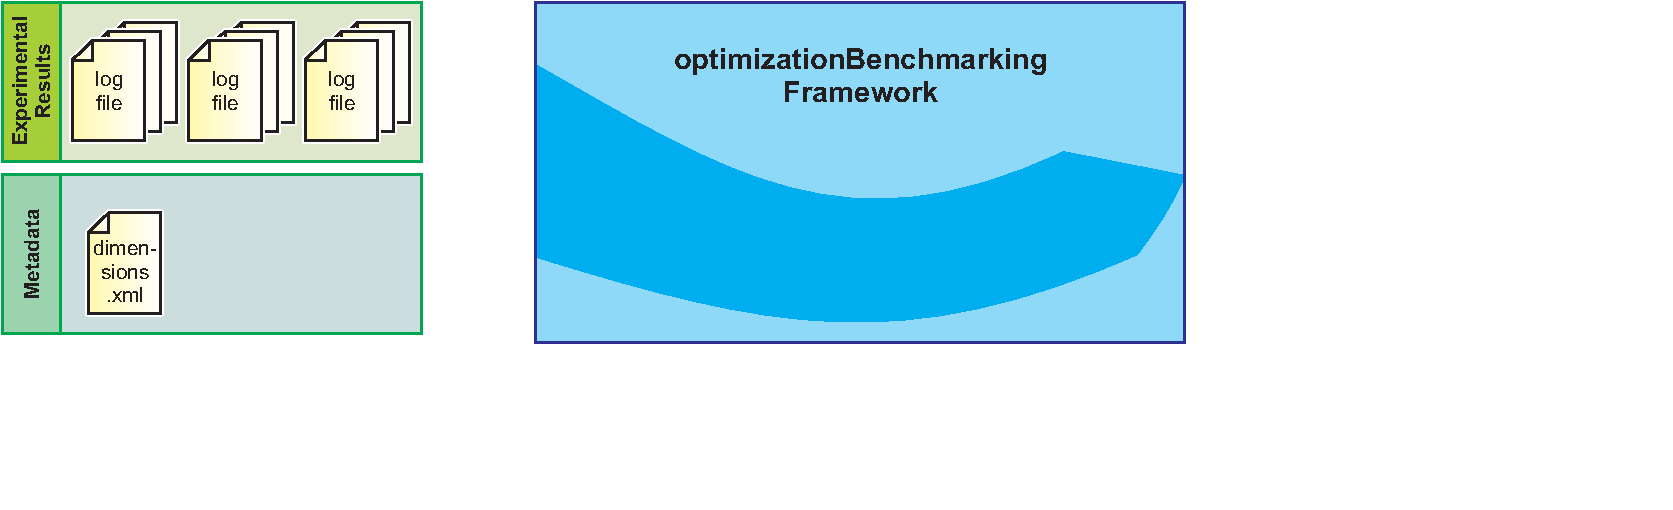
\includegraphics[width=0.9\paperwidth]{graphics/flow/flow_input_2_dimensions}}{0.05}{0.16}%
\locate{6-7}{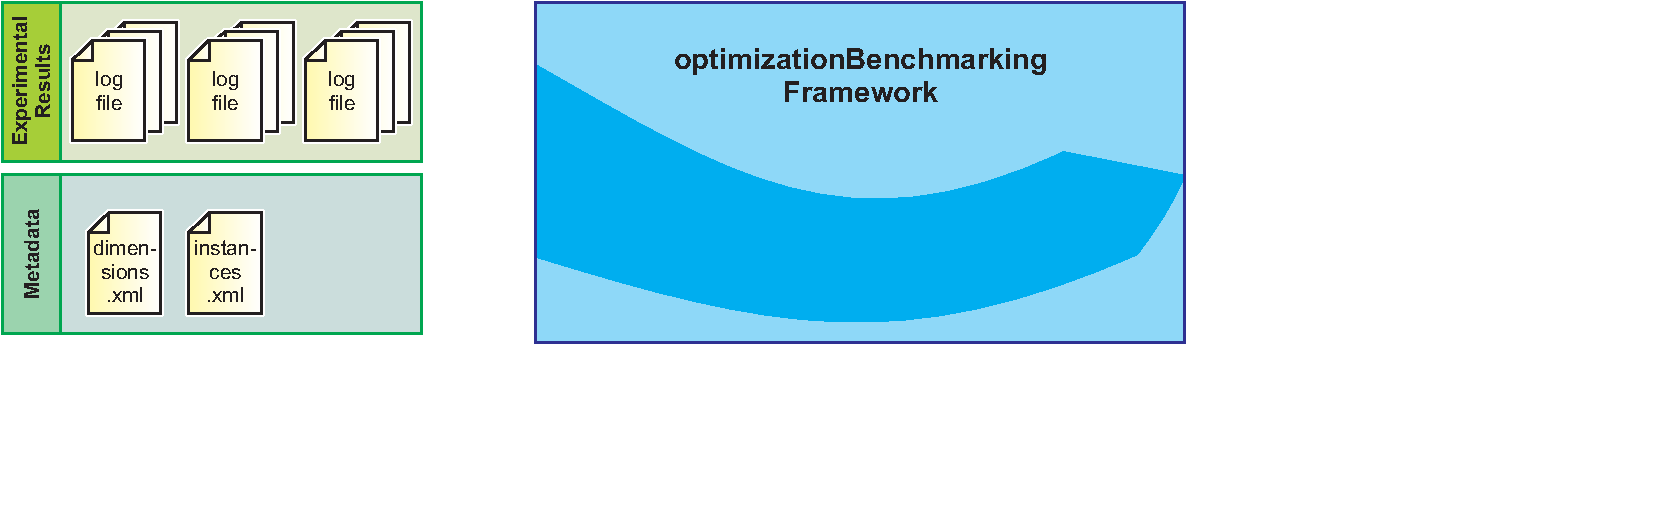
\includegraphics[width=0.9\paperwidth]{graphics/flow/flow_input_3_instances}}{0.05}{0.16}%
\locate{8-9}{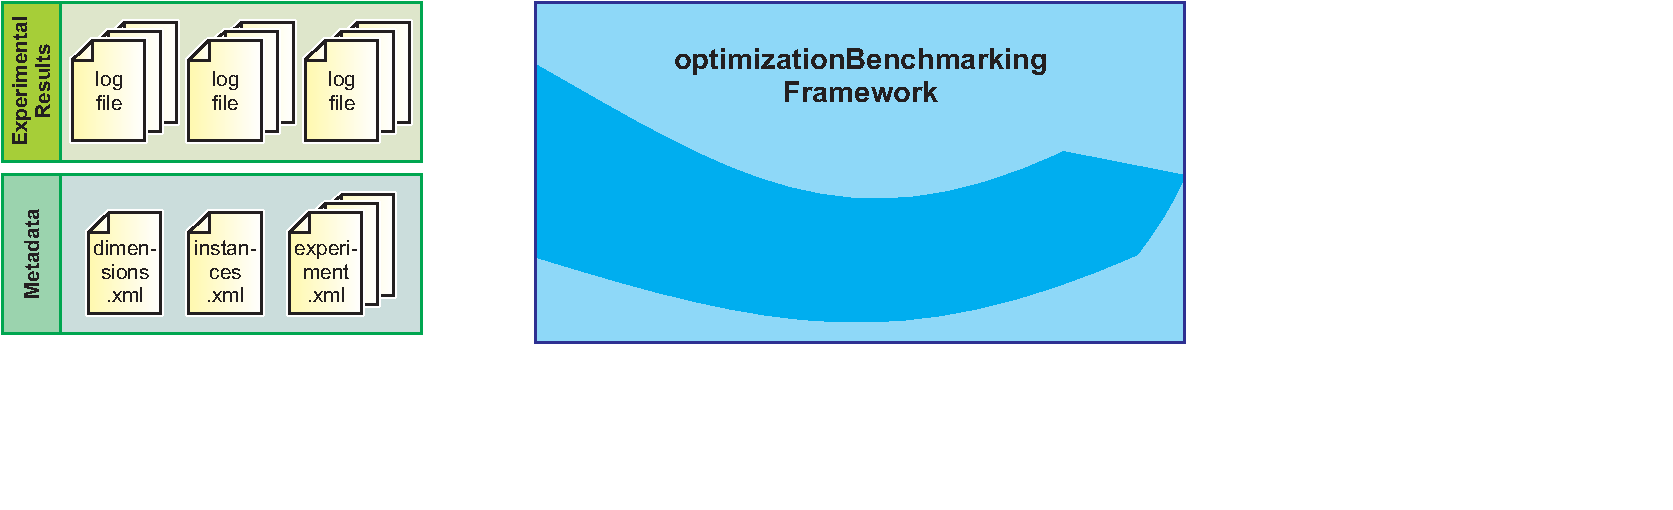
\includegraphics[width=0.9\paperwidth]{graphics/flow/flow_input_4_experiment}}{0.05}{0.16}%
\locate{10-11}{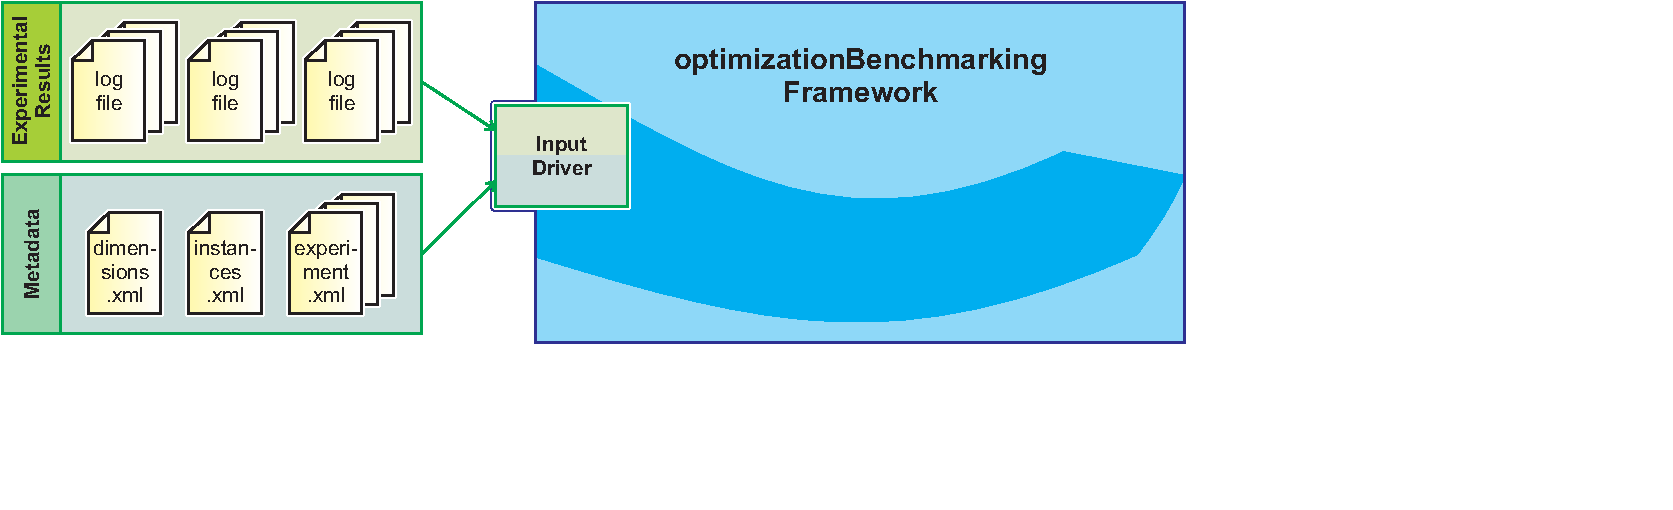
\includegraphics[width=0.9\paperwidth]{graphics/flow/flow_input_5_driver}}{0.05}{0.16}%
\locate{12}{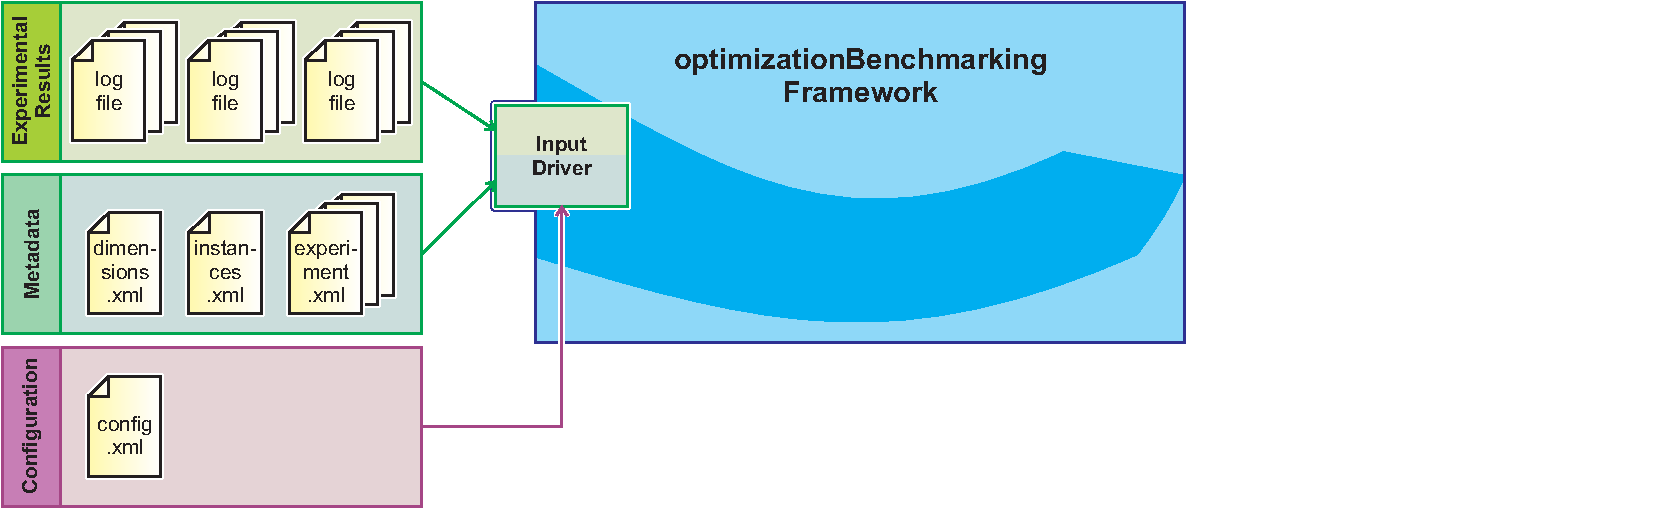
\includegraphics[width=0.9\paperwidth]{graphics/flow/flow_config_1_config}}{0.05}{0.16}%
\locate{13}{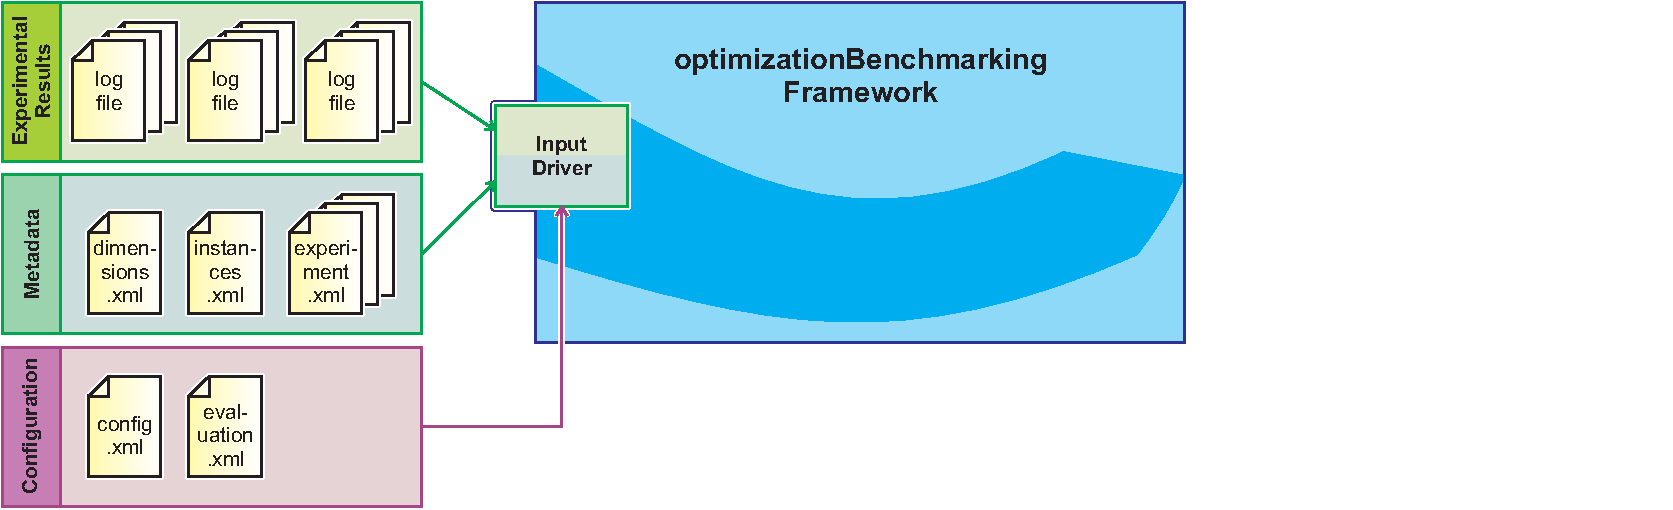
\includegraphics[width=0.9\paperwidth]{graphics/flow/flow_config_2_evaluation}}{0.05}{0.16}%
\locate{14-15}{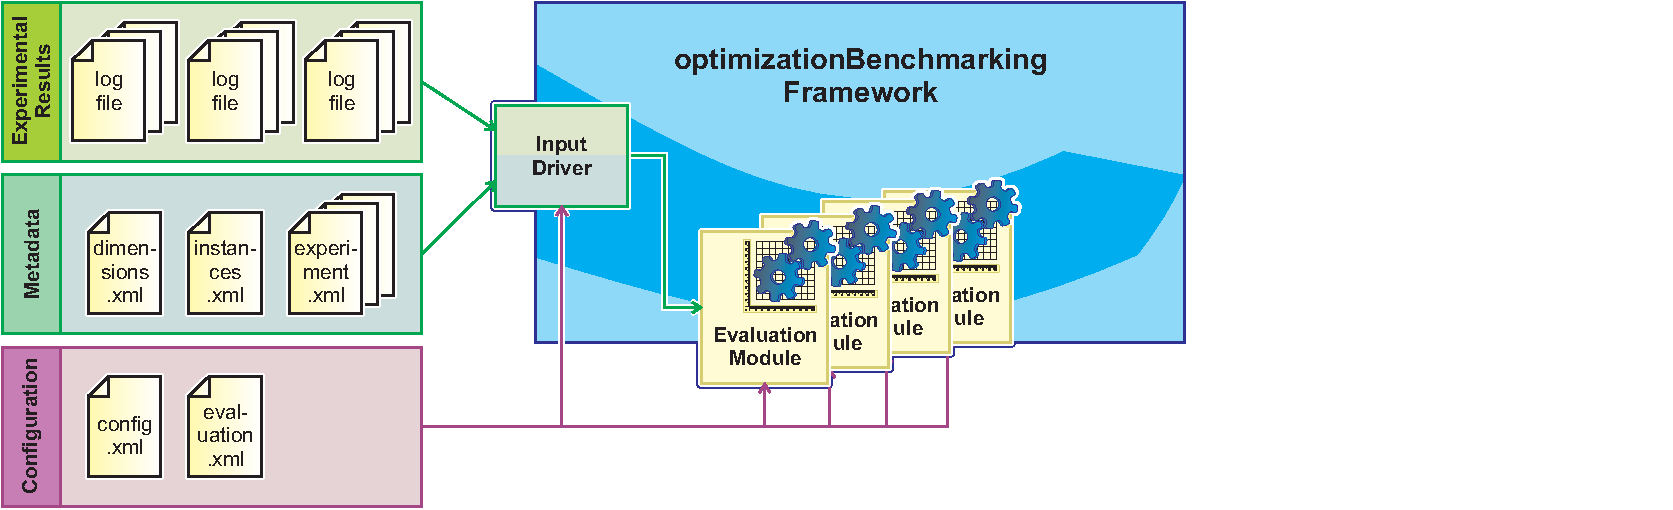
\includegraphics[width=0.9\paperwidth]{graphics/flow/flow_evaluation}}{0.05}{0.16}%
\locate{16}{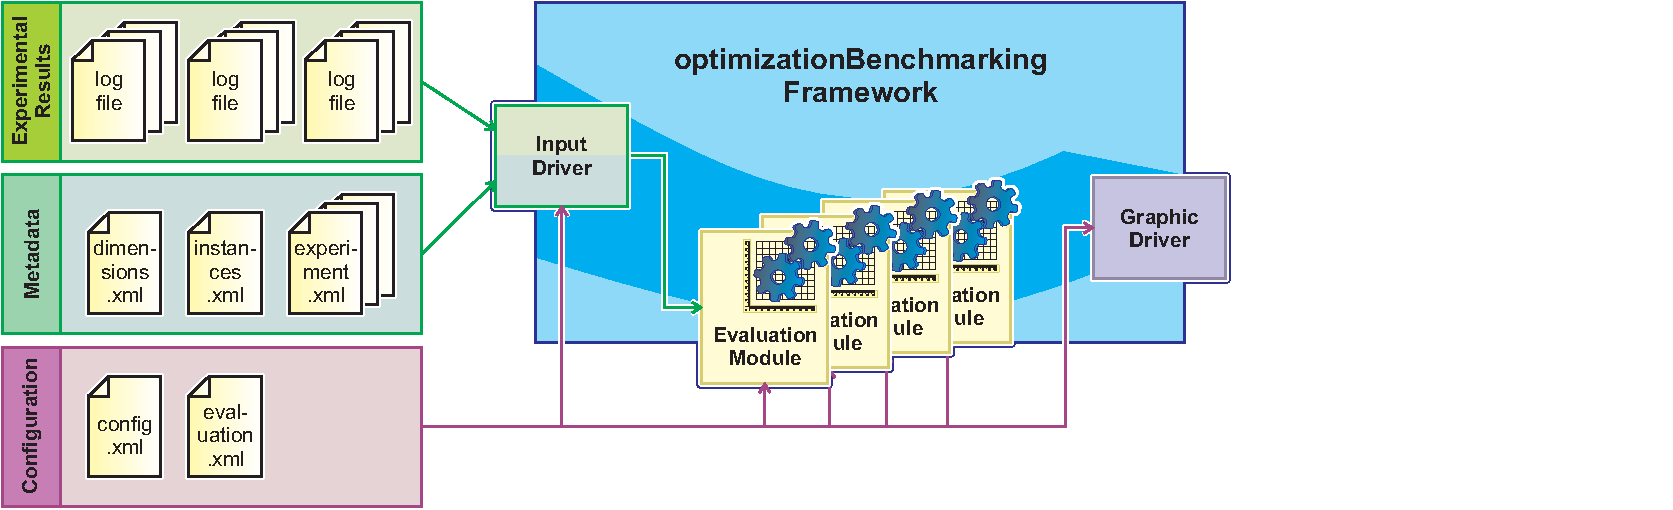
\includegraphics[width=0.9\paperwidth]{graphics/flow/flow_output_1_graphic}}{0.05}{0.16}%
\locate{17}{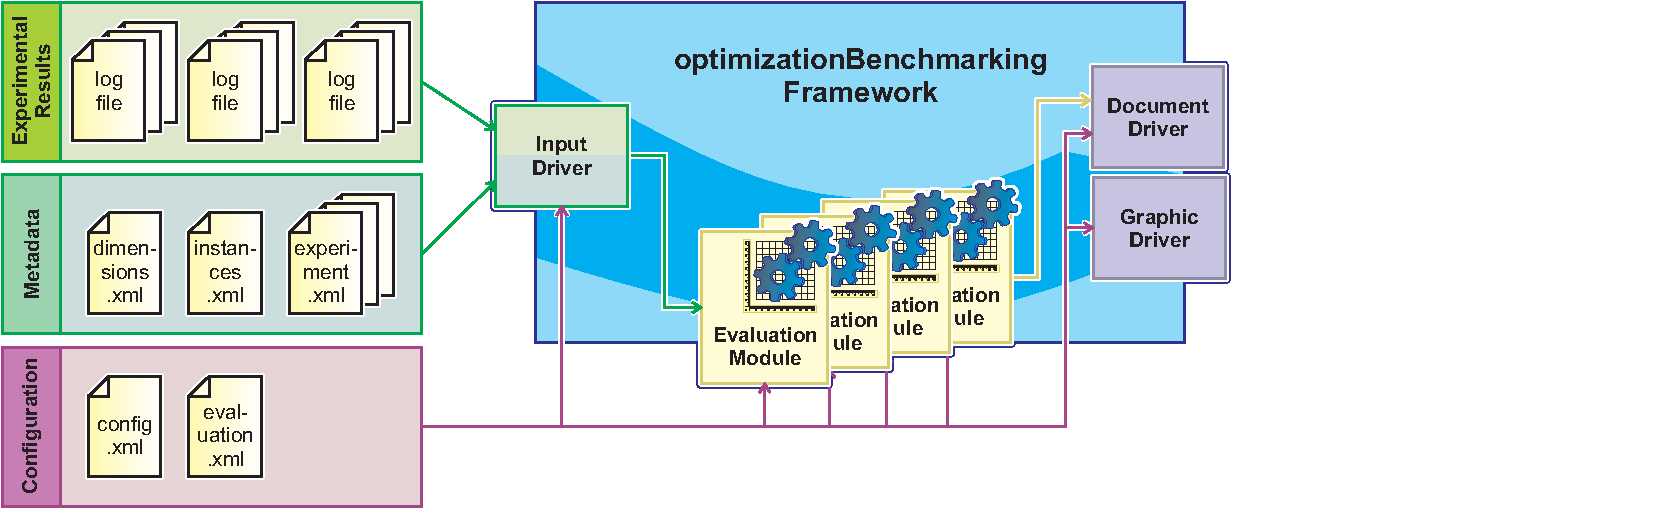
\includegraphics[width=0.9\paperwidth]{graphics/flow/flow_output_2_document}}{0.05}{0.16}%
\locate{18}{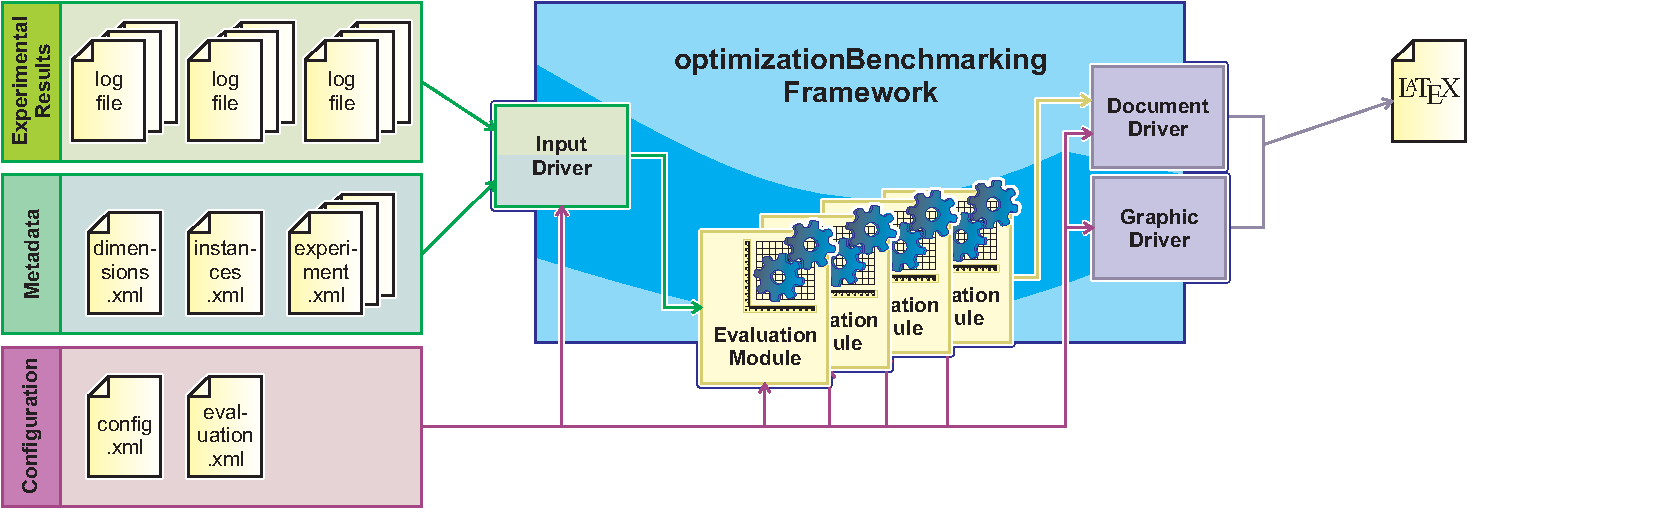
\includegraphics[width=0.9\paperwidth]{graphics/flow/flow_output_3_latex}}{0.05}{0.16}%
\locate{19-21}{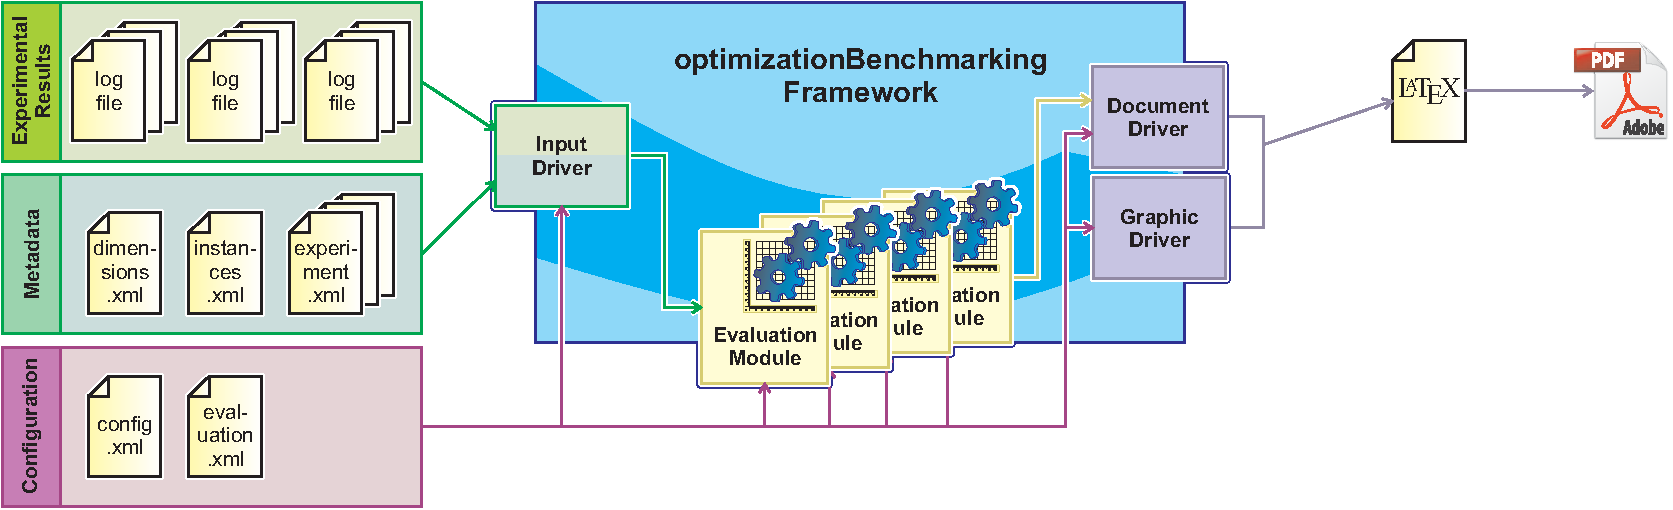
\includegraphics[width=0.9\paperwidth]{graphics/flow/flow_output_4_pdf}}{0.05}{0.16}%
\locate{22}{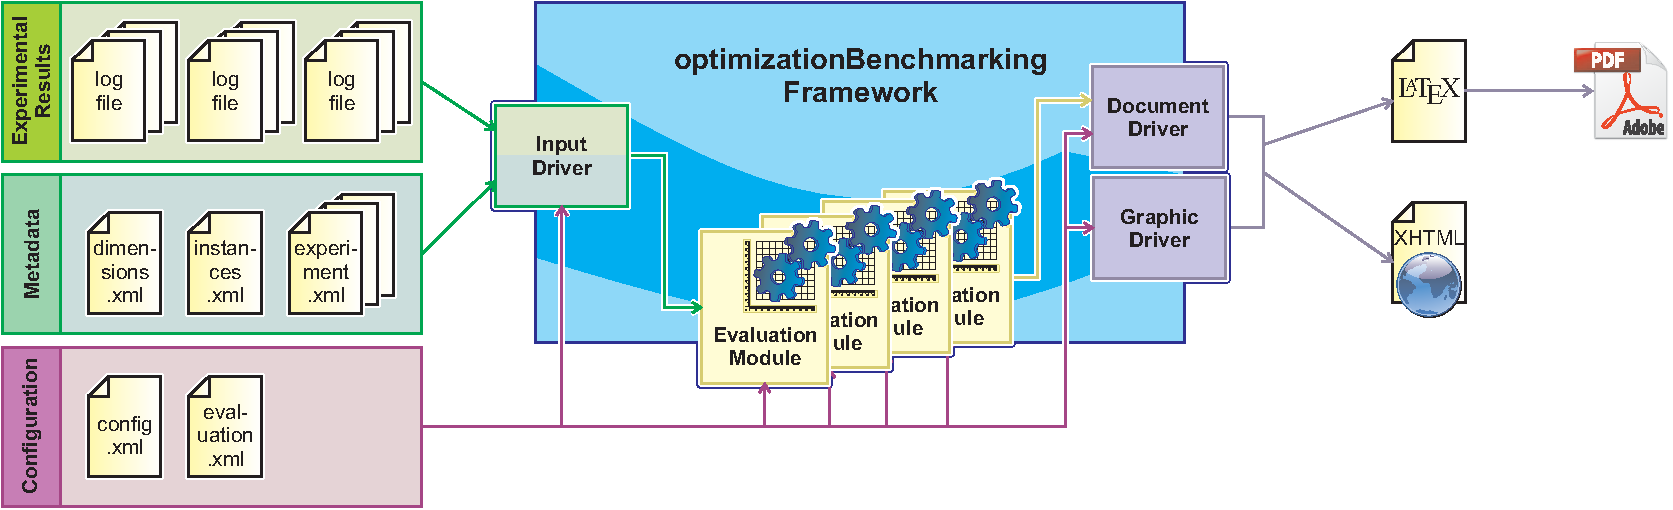
\includegraphics[width=0.9\paperwidth]{graphics/flow/flow_output_5_xhtml}}{0.05}{0.16}%
\locate{23-}{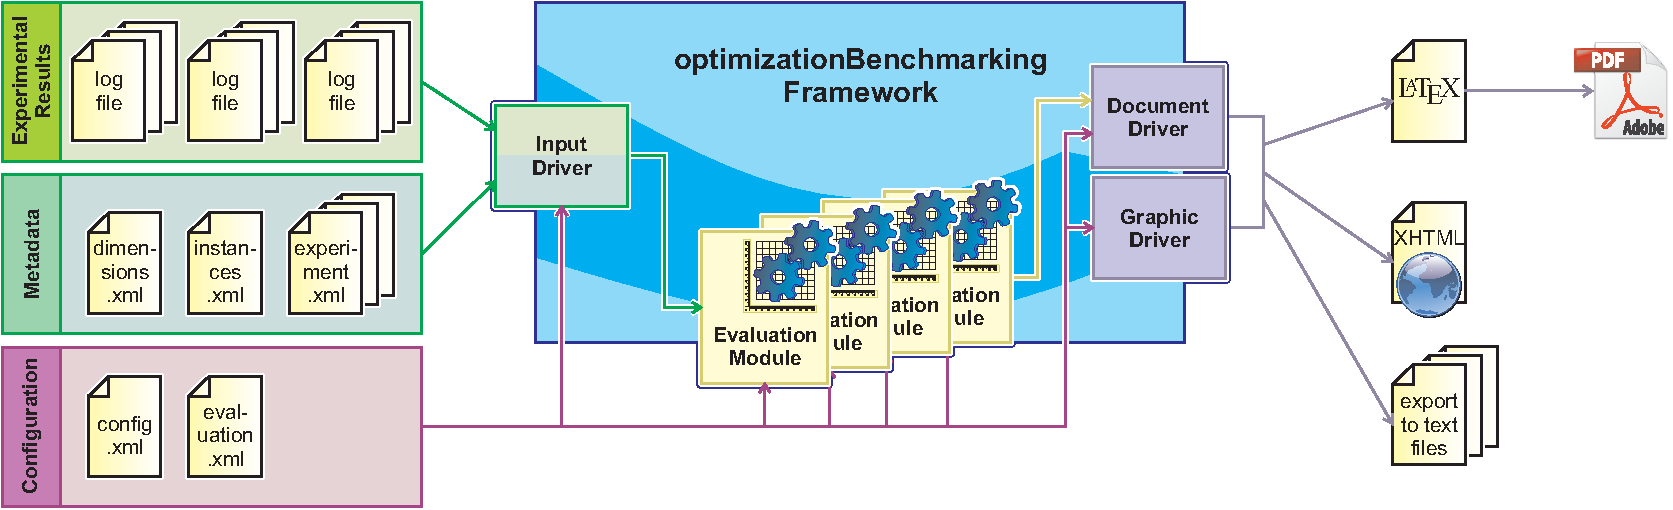
\includegraphics[width=0.9\paperwidth]{graphics/flow/flow}}{0.05}{0.16}%
%
\only<2->{%
\begin{small}%
\begin{itemize}%
%
\only<-9>{%
\item We got a couple of log files for each experiment\uncover<3->{: 6 experiments in our example, each with $10\times 10\times 20=\numprint{2000}$ log files}%
%}%
%
%\only<4-5>{%
\item<4-> We specify which dimensions we have measured\uncover<5->{: \measureFEs, \measureRuntime, and \measureObjectiveValue\ in our example\uncover<-5>{ (\alert{demo})}}%
%}%
%
%\only<6-7>{%
\item<6-> We specify which benchmark instances we have and what their features are\uncover<7->{: $10\times 10$ instances in our example, with features \maxSatVariables\ and \maxSatClauses\uncover<-7>{ (\alert{demo})}}%
%}%
%
%\only<8-9>{%
\item<8-> For each experiment, we specify the parameters\uncover<9->{: in our example, these are \texttt{algorithm}, \texttt{operator}, \texttt{restart}\uncover<-9>{ (\alert{demo})}}%
}%
%
\only<10-13>{%
\item<10-> An \inQuotes{input driver} loads the data\uncover<11->{: most commonly, the data will be in Comma-, Tab-, or Space-Separated-Values format (\textit{CSV}), but we also support \bbob\expandafter\scitep{\bbobReferences} and \tspSuite\expandafter\scitep{\tspSuiteReferences}}%
%}%
%
%\only<12>{%
\item<12-> Via a configuration file, we choose which input and output formats to use, as well as which file specifies the evaluation process%
%}%
%
%\only<13>{%
\item<13-> The \texttt{evaluation.xml} specifies \emph{how} to evaluate the data, i.e., which evaluation modules to apply%
}%
%
\only<14-15>{%
\item<14-> An evaluation module prints on particular type of information about an experiment or experiment set, such as the ECDF, or a table with final results, etc\dots%
\item<15-> Evaluation modules can be applied multiple times, with different configurations (e.g., we can plot ECDFs for different target solution qualities)%
}%
%
\only<16>{%
\item<16-> We can choose among several different formats to be used for graphics, including EPS\scitep{A1992EPFFS}, PDF\scitep{ISO320002008}, PGF (\LaTeX), SVG(Z), EMF, PNG\scitep{RFC2083}, GIF\scitep{CI1990GIFV8}, BMP, and JPG%
\\\strut%
\vspace{0.19\paperheight}%
\strut\\%
}%
%
%
\only<17-21>{%
\item<17-> We can also choose among different formats for the report documents, including\only<-17>{\dots}%
%
\uncover<18-21>{ %
\LaTeX\scitep{MGBCR2004TLC,GMS1994TLC,L1994LADPSUGARM,OPHS2011TNSSITLOLI1M}\uncover<19->{:%
\begin{itemize}%
\item can automatically be compiled to PDF\scitep{ISO320002008}, if a \LaTeX\ compiler (such as TeXLive\scitep{TEXLIVE} or MiKTeX\scitep{MIKTEX}) is auto-detected%
\item<20-> different document classes, such as IEEEtran\scitep{IEEETRAN}, Springer LLNCS\scitep{SPRINGERLNCS}, ACM sig-alternate\scitep{ACMSIGALTERNATE} can be chosen%
\item<21-> graphic sizes and fonts used in graphics are automatically adapted to document class%
\end{itemize}%
}}%
}%
%
\only<22->{\only<-27>{%
\item<22-> We can also choose among different formats for the report documents, including \LaTeX\only<23->{, }\only<-22>{ and }XHTML\scitep{W3C2010XHTML}%
\only<22>{ for quick viewing in a browser}%
\only<23->{, and a plain text format to export results to other applications}}%
%
\item<24-> Evaluation Modules as well as Input, Document, and Graphic Drivers can easily be added\uncover<25->{: %
implement the corresponding interface%
\uncover<26->{%
, put your class into the classpath%
\uncover<27->{%
, and tell the system to use it in the \texttt{config.xml} or \texttt{evaluation.xml}\dots%
%
\only<28->{%
\item<28-> GUI has simple editors and help for all setup, configuration, and meta-data%
}%
%
}}}%
\only<22>{%
\strut\\\medskip\strut%
}%
\only<23->{%
\strut\medskip\strut%
}%
}%
%
\end{itemize}%
\end{small}}%
%
\end{frame}%
%
%
\begin{frame}%
\frametitle{Usage Summary}%
\begin{enumerate}%
\item Implement your optimization or Machine Learning or whatever algorithm%
\item<2-> Select a well-known set of benchmark instances%
\item<3-> Run experiments and obtain one output folder per experiment with log files\medskip%
\item<4-> Put \texttt{dimensions.xml} into results folder (write it with the GUI)%
\item<5-> Put \texttt{instances.xml} into results folder (write it with the GUI)%
\item<6-> Put one \texttt{experiment.xml} into each experiment output folder (write it with the GUI)%
\item<7-> Define your evaluation process in a file \texttt{evaluation.xml} (write it with the GUI)%
\item<8-> Execute \optimizationBenchmarking\ evaluator%
\end{enumerate}%
\end{frame}%
%